%\documentclass[12pt,PhD,twoside]{muthesis}
%\usepackage{verbatim}
%\usepackage{graphicx}
%\graphicspath{ {img/} }
%\usepackage{url} % typeset URL's reasonably
%\usepackage{listings}
%\usepackage{pdfpages}
%\usepackage{tabu}
%\usepackage{longtable}
%\usepackage{multirow, tabularx}
%\usepackage[labelfont=bf]{caption}
%\usepackage{natbib}
%\usepackage{pslatex} % Use Postscript fonts
%\usepackage{amsmath}
%\usepackage{amssymb}
%\usepackage{bm}
%\usepackage{pseudocode}
%\DeclareMathOperator*{\argmin}{arg\,min}
%\DeclareMathOperator*{\argmax}{arg\,max}
%\def\approxprop{%
%	\def\p{%
%		\setbox0=\vbox{\hbox{$\propto$}}%
%		\ht0=0.6ex \box0 }%
%	\def\s{%
%		\vbox{\hbox{$\sim$}}%
%	}%
%	\mathrel{\raisebox{0.7ex}{%
%			\mbox{$\underset{\s}{\p}$}%
%		}}%
%	}
%\begin{document}
%\bibliographystyle{model5-names}

\chapter{Supplementary Information for Chapter 5}
\label{apx:mapstruture}

\section{Tree analysis algorithm}

We used an algorithm to extract map structure from recall orders which is functionally equivalent to the ordered tree algorithm used in prior work (Hirtle \& Jonides, 1985; McNamara, 1986; McNamara et al., 1989), with the exception that we disregard order information (whether or not the leaves were always recalled in a particular ordering). The algorithm takes a list of recall protocols, as well as cues, and all possible buildings, and returns the map structure (all sets of buildings which always occur together).

\begin{pseudocode}[ruled]{ExtractMapStructure}{Protocols, Cues, Buildings}
	1: submaps \GETS \{ \} \\
	2: \FOREACH tuplelength \in (1, |Buildings|-1) \\
	3: \quad \FOREACH C \in Combinations(Buildings, tuplelength) \\
	4: \quad\quad occurseverywhere \GETS True \\
	5: \quad\quad \FOREACH p \in (0, |Protocols|) \\
	6: \quad\quad\quad perm \GETS Permutations(C) \\
	7: \quad\quad\quad \IF Cues[p] \notin C \AND \forall (PC \in perm : PC \notin Protocols[p]) \\
	8: \quad\quad\quad\quad occurseverywhere \GETS False \\
	9: \quad\quad\quad\quad \textbf{break} \\
	10: \quad\quad \IF occurseverywhere \\
	11: \quad\quad\quad submaps \GETS submaps \cup {C}
\end{pseudocode}

The algorithm iterates through all possible tuple lengths, and generates all possible combinations at the current tuple length. For these combinations $C$, it checks whether any permutation of $C$ occurs uninterrupted in all protocols (i.e. whether all buildings in $C$ have been recalled together); if so, $C$ is added to the list of submaps. Notably, this check is only performed if C is not cued (line 7). It was argued in previous literature (Hirtle \& Jonides, 1985; McNamara et al., 1989) that cueing can disrupt the re-call process. Therefore containment in all protocols is only tested for combinations which do not contain a cue, in order to avoid erroneously disregarding sub-maps which consistently occur together in all recall protocols except in those in which the cue has disrupted the natural recall order.

\section{Full list of cities chosen by included subjects}

The map in Figure \ref{fig_map} provides a visual overview over all cities within which spatial memory data has been collected from the participants.

\begin{figure}[h]
	\centering
	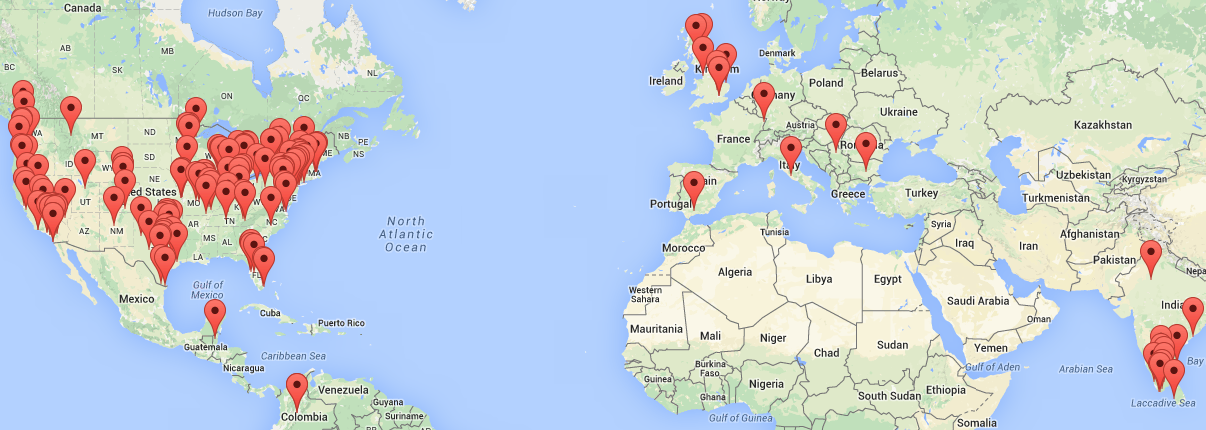
\includegraphics[width=\textwidth]{mapcities.png}
	\caption{Overview over the 149 cities chosen by subjects in Experiments 1, 3A and 3B.}
	\label{fig_map}
\end{figure}

List of cities in Experiment 1: \footnotesize{Albany, Albuquerque, Ames, Ann Arbor, Austin, Baltimore, Belgrade, Belmopan, Buffalo, Chennai, Chicago, Chico, Cincinnati, Corvallis, Cupertino, Denton, Denver, Dunmore, Fort Collins, Gobichettipalayam, Hampton, Klamath Falls, Kochi, Lakeland, Las Vegas, Los Angeles, Madurai, Miami, Minneapolis, Miramar, Mount Kisco, New York, Orange (FL), Pittsburgh, Pittsfield Charter Township, Potterville, Reno, Rome, San Angelo, San Bernardino, San Diego, Somerville, Springfield, Strasbourg, White Salmon, Williamsburg, Wilmington}.

\normalsize

List of cities in Experiment 3A: \footnotesize{Alameda, Austin, Beacon, Bedford, Belleville, Bellingham, Bengaluru, Berkeley, Bloomington, Boston, Bowie, Bowling Green (KY), Brooksville, Brownsville, Buffalo, Burlington, Cambridge, Camden, Cape Girardeau, Castlerock, Chicago, Cincinnati, College Station (TX), Colombo, Columbia, Denver, Desert Hot Springs (CA), Desoto, Duluth, Eastbrunswick, Edinburgh, Fairway, Farmersville, Fayetteville, Franklin, Germantown, Gettysburg, Glasgow, Goleta, Harwoodheights, Hemet, Highridge, Hollywood, Holt, Houston, Islavista, Jaipur, Karur, Keller, Lackawanna, Lake Oswego, Land O' Lakes, Lindsay, Little River-Academy (TX), Live Oak (TX), London, Lubbock, Marthandam, Mayfield, Minneapolis, Mission, Nagercoil, New York, Norridge, Orange, Overland Park (KA), Owensville, Palmsprings, Perryville, Pigeonforge, Poplarbluff, Portland, Poughkeepsie, Princeton, Provo, Revere, Rochester, Rochester Hills, Roeland Park, Salem, San Antonio, San Diego, Sanger, Savage, South Bend, Southport, Springboro, Springhill, St. Charles, Stony Brook (NY), St. Peters, Temple, Tirunelveli, Towson, Visakhapatnam, Warren, Weatherford, Wilmington, Xenia, Ypsilanti}.

\normalsize

List of cities in Experiment 3B: \footnotesize{Algonquin, Ashland, Chicago, Columbia, Jefferson City, Kansas City, Knoxville, Lexington, Linden, Medford, Minneapolis, Missoula, Mound, Overland Park, Portland, Seattle, Stara Zagora}.

\normalsize

\section{Exclusion of learning effects}

A possible criticism of our results could be the claim that the structure apparent from the recall protocol orderings is being learned by the subjects during the recall process, as opposed to being an inherent property of their long-term memory (LTM). Our analysis procedure assumes one consistent structure in LTM underlying the recall protocols; and excludes possible `outliers' using the jackknifing procedure (i.e. protocols which, when included, would statistically significantly change the resulting structure, are excluded from analysis).

If this assumption was incorrect, and subjects learned the structure during the experiment - or, alternatively, re-learned a different structure, then this would be apparent from the pattern of omitted recall protocols. Specifically, it would mean a significantly larger number of omitted early protocols compared to late protocols (the first few protocols would be inconsistent with the learned structure more often than the last few).

To test whether this learning effect can be observed, we have tested the distributions of omitted recall protocols against the null hypothesis that the likelihood of omissions was uniform (just as likely to occur for the first few as for the last few protocols), using a chi-square test. The table below shows the results. 

For the real-world experiments, the null hypothesis cannot be rejected; thus, it is likely that there is no learning effect, and that our recall order paradigm indeed measures structures which have already been committed to LTM before the experiment. For the virtual reality experiment (Exp. 2), there seems to be some small non-uniformity, although not significant at $\alpha=0.01$. However, contrary to the objection that the structure arises from learning during the recall trials, early protocols were less likely \footnote{The frequency of omissions in Experiment 2 were: $1.1\%$ for the protocols presented first, $0.7 \%$ for those at position 2, $1.3\%$ at position 3, $1.6\%$ at position 4, $1.7\%$ at position 5, $1.9\%$ at position 6, and $1.8\%$ at position 7}, instead of more likely, to be excluded as outliers compared to late protocols. 

\begin{table}
	\centering
	\begin{tabularx}{\textwidth}{XXXX}
		\textbf{Exp. 1} & \textbf{Exp. 2} & \textbf{Exp. 3A}  & \textbf{Exp. 3B} \\ \hline
		$p=0.886 > 0.01$ & $p=0.015 > 0.01$ & $p=0.146 > 0.01$ & $p=0.495 > 0.01$  \\
		$c=2.339$ & $c=15.698$ & $c=9.538$ & $c=8.393$  \\ \hline
		%		\small{No evidence for \newline non-uniformity} & \small{Weak evidence for \newline non-uniformity} & \small{No evidence for \newline non-uniformity} & \small{No evidence for \newline non-uniformity} \\
	\end{tabularx}
	\caption[Results of chi-squared tests against the null hypothesis that there is no learning effect in the recall protocol data]{Results of chi-squared tests against the null hypothesis that there is no learning effect in the recall protocol data, i.e. that early recall protocols are as likely to be outliers than late recall protocols ($p$ is the p-value of the test; $c$ denotes the chi square test statistic). The non-significance of the results suggests that our recall order paradigm measures a property of long-term memory, and not something learned during the recall trials.}
	\label{tbl_chisq}
\end{table}

\section{Separability of co-represented and not co-represented building pairs}

The co-representation correlations reported in Section 3.3 of the main text raise hopes of straightforward predictability - what if a simple distance thresholding or linear decision boundary in the reported feature space is capable of fully explaining cognitive map structure, even for the random testing environments? Unfortunately, within sub-map and across sub-map building pairs are not linearly separable; and difficult to separate in general, even with complex state of the art classifiers. 

% (the Supplementary Information contains dimensionality-reduced plots of the pair distributions). We have tried several state of the art classification algorithms from machine learning, including kernel Support Vector Machines and Random Forests.

\begin{figure}[h]
	\centering
	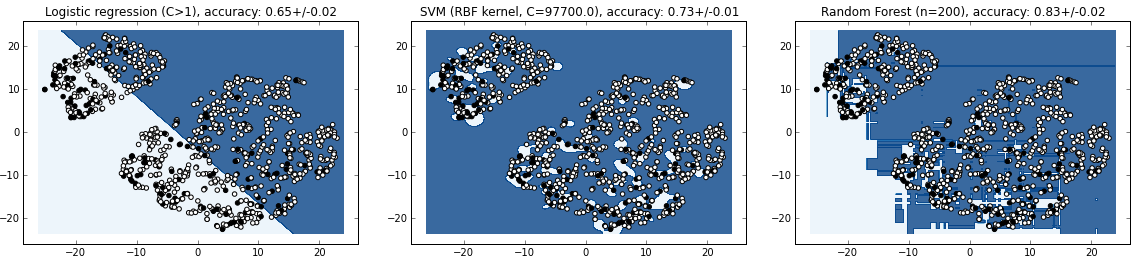
\includegraphics[width=\textwidth]{exp2class.png}
	\caption[Pairs of buildings in the space of all features, and separability, in Experiment 2]{Pairs of buildings in the space of all features, and separability according to co-representation, in Experiment 2 using 3 different classifiers: logistic regression (left), Support Vector Machine with RBF-kernel (middle) and Random Forest (right). Each point represents a building pair (filled black if both buildings lie on the same sub-map, and white if they do not), with its position being a two-dimensional projection of the full six-dimensional feature space using t-SNE.  Although 2D decision boundaries are visualized, the reported classifier accuracies were obtained in the original feature space, using 10-fold cross validation and after hyperparameter optimization.}
	\label{fig_classify}
\end{figure}

\begin{figure}[h]
	\centering
	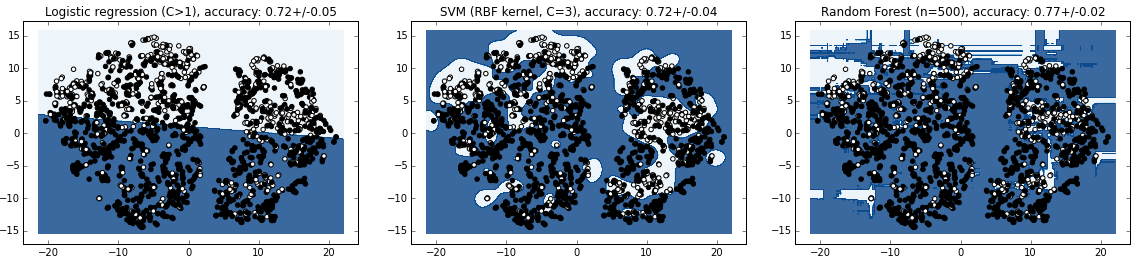
\includegraphics[width=\textwidth]{exp3Aclass.png}
	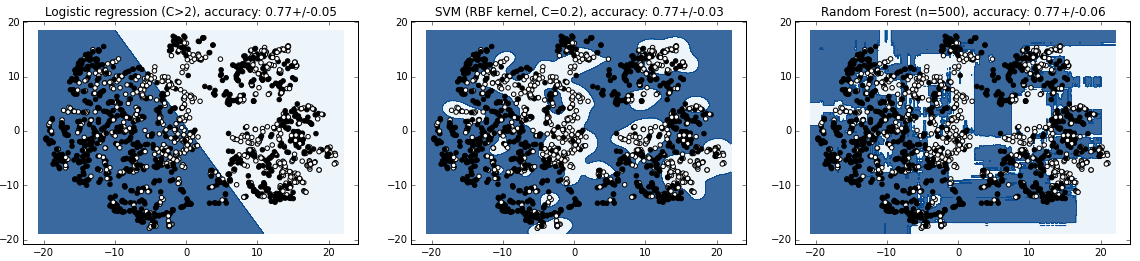
\includegraphics[width=\textwidth]{exp3Bclass.png}
	\caption[Pairs of buildings in the space of all features, and separability, in Experiment 3]{Pairs of buildings in the space of all features, and their separability according to co-representation, in Experiment 3 using three different classifiers: logistic regression (left), Support Vector Machine with RBF-kernel (middle) and Random Forest (right). Top: Condition A. Bottom: Condition B}
	\label{fig_classify_rl}
\end{figure}

Figure \ref{fig_classify} shows the distances of all pairs of buildings in all features in Experiment 2, normalized by dividing each feature by its standard deviation for each participant map, and compressed down to two-dimensional space for visualization using t-SNE (without normalization across buildings of each map, classifiers are unable to perform above chance). Apart from the building pairs (which concentrate into two groups according to function - shops and houses), decision boundaries obtained with three different classifiers are also plotted. Although there is a trend of building pairs being more likely to be on the same sub-map when closer together (higher concentration of same-map pairs towards the lower left), the data is clearly not well-separable. As can be seen from this Figure, accurate prediction of full subject map structures - or even whether single building pairs belong to the same sub-map - using simple classification is impossible using naive approaches. More complex machine learning algorithms such as random forests (state-of-the art classifiers based on ensembles of decision trees) (Breiman, 2001) can predict for around $83 \%$ of building pairs whether they belong to the same representation (note that the accuracies were obtained by classifying the full high-dimensional data set, not just the 2D projection plotted in Figures \ref{fig_classify} and \ref{fig_classify_rl}). However, the map structures collected in our experiments contain $10$ and $28$ pairs (in the $5$-building and $8$-building maps), which would make the probability of full map structures - all pairs - being predicted correctly using this approach $15.5 \%$ and $0.5 \%$ respectively (the situation is even worse in real-world environments, as can be seen in the next section).

In the more complex real-world setting of Experiment 3, separating pairs of buildings which belong to the same sub-map and those belonging to different sub-maps is even more difficult than in virtual reality environments, as shown by Figure \ref{fig_classify_rl} and evidenced by the lower accuracies obtained after 10-fold cross validation. This Figure shows the distances of all pairs of buildings in all features, normalized by dividing each feature by its standard deviation for each participant map, and compressed down to two-dimensional space for visualization using t-SNE. Note that the Figure shows prediction accuracies of pairs of buildings (whether or not a pair was represented on the same sub-map), and not of entire map structures. To correctly predict a map structure, all pairs within would need to be predicted correctly. Given the $77 \%$ accuracy of the best classifier in Figure \ref{fig_classify_rl}, correct predictions based on classification are even more unlikely than in Experiment 2 ($0.77^{5 \choose 2}=7.3 \%$ in condition A, and $0.77^{8 \choose 2}=0.0 \%$ in condition B).

%Due to the large number of trees - $N=200$ -, this approach is able to learn decision trees describing regions in this feature space for each individual participant, which is why it performs better than the other approaches.


%\footnote{Logistic regression performed equally with l1 and l2 regularization, and with any regularization parameter C greater than 1}

%The observation that building pair classification fails altogether \footnote{All approaches yield accuracies around $50\%$ for binary, within vs. between sub-map classification for unnormalized data} when distances are not normalized across buildings of each map (within each subject and environment) provides an important hint as to the reason of why classification is a sub-optimal approach to model and predict cognitive map structure. It implies that \textit{relative} distances are much more relevant than absolute distances. This is another argument in favour of the clustering hypothesis, since in clustering, relative distances are the sole criterion of cluster structure. Furthermore, it illustrates the difficulty of the problem, and the inadequacy of naive approaches for solving it.

%
%\begin{thebibliography}{5}
%	\expandafter\ifx\csname natexlab\endcsname\relax\def\natexlab#1{#1}\fi
%	\providecommand{\url}[1]{\texttt{#1}}
%	\providecommand{\href}[2]{#2}
%	\providecommand{\path}[1]{#1}
%	\providecommand{\DOIprefix}{doi:}
%	\providecommand{\ArXivprefix}{arXiv:}
%	\providecommand{\URLprefix}{URL: }
%	\providecommand{\Pubmedprefix}{pmid:}
%	\providecommand{\doi}[1]{\href{http://dx.doi.org/#1}{\path{#1}}}
%	\providecommand{\Pubmed}[1]{\href{pmid:#1}{\path{#1}}}
%	\providecommand{\bibinfo}[2]{#2}
%	\ifx\xfnm\relax \def\xfnm[#1]{\unskip,\space#1}\fi
%	%Type = Article
%	\bibitem[{Breiman(2001)}]{breiman2001random}
%	\bibinfo{author}{Breiman, L.} (\bibinfo{year}{2001}).
%	\newblock \bibinfo{title}{Random forests}.
%	\newblock {\it \bibinfo{journal}{Machine learning}\/},  {\it
%		\bibinfo{volume}{45}\/}, \bibinfo{pages}{5--32}.
%	%Type = Article
%	\bibitem[{Hirtle \& Jonides(1985)}]{Hirtle_Jonides_1985}
%	\bibinfo{author}{Hirtle, S.}, \& \bibinfo{author}{Jonides, J.}
%	(\bibinfo{year}{1985}).
%	\newblock \bibinfo{title}{Evidence of hierarchies in cognitive maps}.
%	\newblock {\it \bibinfo{journal}{Memory \& Cognition}\/},  {\it
%		\bibinfo{volume}{13}\/}, \bibinfo{pages}{208--217}.
%	%Type = Article
%	\bibitem[{Van~der Maaten \& Hinton(2008)}]{van2008visualizing}
%	\bibinfo{author}{Van~der Maaten, L.}, \& \bibinfo{author}{Hinton, G.}
%	(\bibinfo{year}{2008}).
%	\newblock \bibinfo{title}{Visualizing data using t-sne}.
%	\newblock {\it \bibinfo{journal}{Journal of Machine Learning Research}\/},
%	{\it \bibinfo{volume}{9}\/}, \bibinfo{pages}{85}.
%	%Type = Article
%	\bibitem[{McNamara(1986)}]{mcnamara1986mental}
%	\bibinfo{author}{McNamara, T.~P.} (\bibinfo{year}{1986}).
%	\newblock \bibinfo{title}{Mental representations of spatial relations}.
%	\newblock {\it \bibinfo{journal}{Cognitive psychology}\/},  {\it
%		\bibinfo{volume}{18}\/}, \bibinfo{pages}{87--121}.
%	%Type = Article
%	\bibitem[{McNamara et~al.(1989)McNamara, Hardy \&
%		Hirtle}]{mcnamara1989subjective}
%	\bibinfo{author}{McNamara, T.~P.}, \bibinfo{author}{Hardy, J.~K.}, \&
%	\bibinfo{author}{Hirtle, S.~C.} (\bibinfo{year}{1989}).
%	\newblock \bibinfo{title}{Subjective hierarchies in spatial memory.}
%	\newblock {\it \bibinfo{journal}{Journal of Experimental Psychology: Learning,
%			Memory, and Cognition}\/},  {\it \bibinfo{volume}{15}\/},
%	\bibinfo{pages}{211}.
%	
%\end{thebibliography}



%\bibliography{mapstructure}
%\end{document}